\documentclass[a4paper,twocolumn]{article}

\usepackage{graphicx}          % To handle figures
\usepackage{amsmath}           % Defines certain mathematical symbols
%\usepackage{psfrag}            % Inserts LaTeX text into figures (does not work with PDFLatex)

% Makes sure that all Swedish characters
                               % work
%\usepackage[swedish]{babel}    % If you want to write in Swedish.

\addtolength{\topmargin}{-25mm}% Decrease the top margin by 25mm
\addtolength{\textheight}{25mm}% Increase the text height by the
                               % same amount

\begin{document}

\title{Bank filtering for sound compression}
\author{Baptiste Cavarec \\ 940321-T197 \and Hugo Lime\\
  Personalnumber2}
%\date{2000-10-10} % If you don't want todays date.

\maketitle


\begin{abstract}
  The summary/abstract is perhaps the most important part of a
  report. Here you should catch the attention of the reader. Bring up
  the problem you want to solve and briefly summarize your results.
\end{abstract}

\section{Introduction}
\label{sec:intro}

In this project, we intend to study the common problematic of data compression,in our case for sound signals. We have as an input a sound signal sampled at a 8 kHz frequency. In order to store and compress our signal, we need to implement an analysis filter bank.The one we decided to implement can be seen in Fig.~\ref{fig:analysis}. As one can also see in Fig.~\ref{fig:analysis}, we also compute quantization of our 3 signals obtained by the analysis. This is the core of our data storage issue, as we need to quantize in order to lower the signal's data rate. This obviously induces quantization noise and deteriorates the signal, we then have to find the best way to avoid the noise.

\begin{figure}[!ht]
  \begin{center}
    % Standard LaTeX can handle EPS files.
    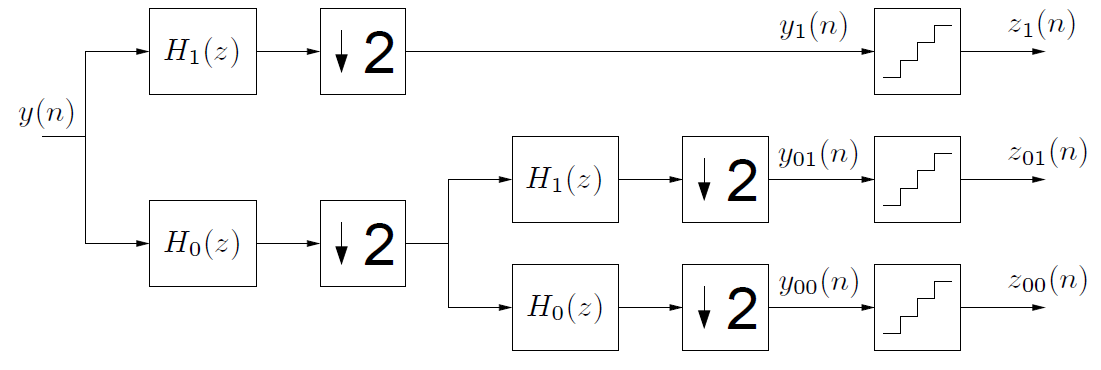
\includegraphics[width=0.83\columnwidth]{analysis.png}
    % If you instead use pdflatex to process the file, the
    % figures should be in PDF, JPG or PNG format.
  \end{center}
  \caption{Analysis filter bank followed by quantization.}
  \label{fig:analysis}
\end{figure}

Then, we use the synthesis filter bank presented in Fig.~\ref{fig:synthesis} in order to reconstruct the signal. Sec.~\ref{sec:reconstruction} will present the filters used and their impact on the signal.

\begin{figure}[!ht]
  \begin{center}
    % Standard LaTeX can handle EPS files.
    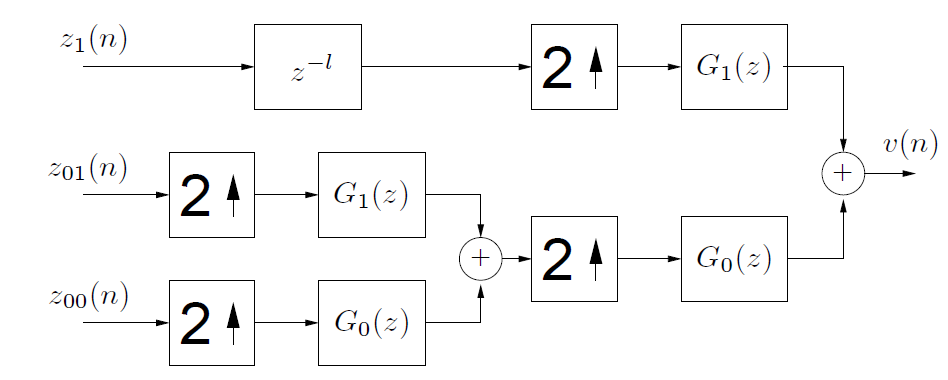
\includegraphics[width=0.83\columnwidth]{synthesys.png}
    % If you instead use pdflatex to process the file, the
    % figures should be in PDF, JPG or PNG format.
  \end{center}
  \caption{Synthesis filter bank.}
  \label{fig:synthesis}
\end{figure}

In order to evaluate the error introduced by the above mentioned quantization scheme, we need to introduce a measure of our quantization/reconstruction scheme efficiency as Sec.~\ref{sec:reconstruction} ensures perfect reconstruction, this measure would only seize the impact of the quantization on the compressed sound.
The measure we consider is called Signal to Quantification Noise Ratio (SQNR) and can be evaluated as in Eq.~\ref{eq:sqnr}. 
\begin{equation}
  \label{eq:sqnr}
  SQNR= \frac{E[y^2]}{E[\left(y-v\right)^2]}
\end{equation}




\section{Theory}
\label{sec:theory}
\subsection{Bank filtering}
\label{sec:reconstruction}
We presented in Sec.~\ref{sec:intro}, our structure is based on Analysis/Synthesis Filter Bank scheme (Fig.~\ref{fig:analysis} and Fig.~\ref{fig:synthesis}).
In order to ensure the reconstruction of our signal, we need to design the filters so that they respect Eq.~\ref{eq:filters1}.\begin{equation}
  \label{eq:filters1}
H_1(z)=G_0(-z)
\end{equation}
\begin{equation}
G_1(z)=-H_0(-z)		
\end{equation}
\begin{equation}
\label{eq:condh0g0}
G_0(z)H_0(z)-G_0(-z)H_0(-z)=2\cdot z^{-l}		
\end{equation}
 Moreover, in order to perform the synthesis scheme, we need to know the delay introduced by or Analysis/Synthesis bank. By using the formalism presented in Eq.~\ref{eq:g0h0} we ensure a delay $l=3$ for our "first order" filter bank, if Q is an order 2 polynomial in $z^{-1}$. If we want to ensure that Eq.~\ref{eq:condh0g0} is satisfied, we must have $Q(z)=-\frac{1}{16}+\frac{z^{-1}}{4}-\frac{z^{-2}}{16}$, a demonstration of this result can be found at Appendix~\ref{sec:demoQ}.
\begin{equation}
  \label{eq:g0h0}
G_0(z)H_0(z)=(1+z^{-1})^4Q(z)
\end{equation}
Given this, we choose $G_0(z)=\frac{1}{2}\left(1+z^{-1}\right)^2$ it then leads to $H_0(z)=\frac{1}{8}\left(-1+2z^{-1}+6z^{-2}+2z^{-3}-z^{-4}\right)$. Hence, $H_1(z)=\frac{1}{2}\left(1-z^{-1}\right)^2$ and $G_1(z)=-\frac{1}{8}\left(-1-2z^{-1}+6z^{-2}-2z^{-3}-z^{-4} \right)$.

Fig.~\ref{fig:filters} shows the shape of these filters in frequency domain.


\begin{figure}[!ht]
  \begin{center}
    % Standard LaTeX can handle EPS files.
    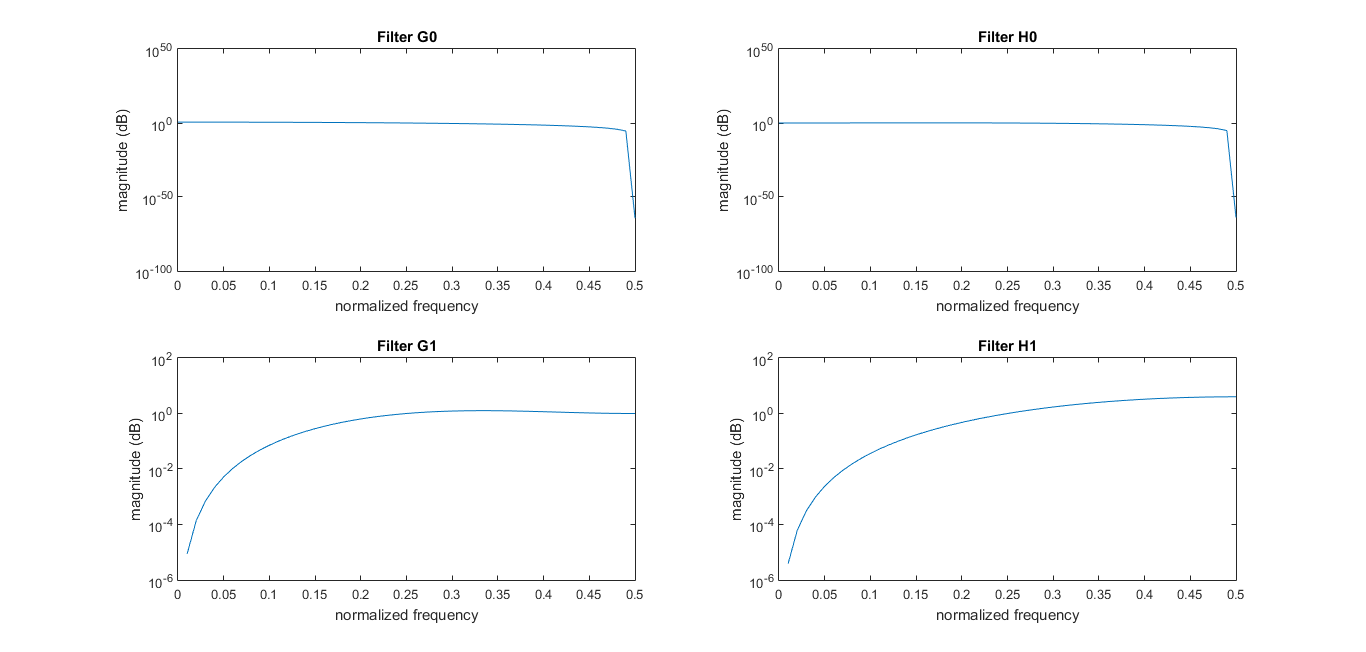
\includegraphics[width=1.1\columnwidth]{filters.png}
    % If you instead use pdflatex to process the file, the
    % figures should be in PDF, JPG or PNG format.
  \end{center}
  \caption{Frequency response of the filters used in our Analsys/Synthesis scheme}
  \label{fig:filters}
\end{figure}


Given this we will ensure in Sec.~\ref{sec:numreconstruction} that these filters performs perfect reconstruction.


\subsection{Total delay of the system}
Once one have seen on Sec.~\ref{sec:reconstruction} we introduce a delay by implementing these filters. The delay introduce by the "first order" Analysis/Synthesis scheme is given and is $l=3$. Given this one may see that we use this scheme twice including in the downsampled part of our system. The outsampling would result on a $2 \cdot 3$ delay in the normal part of the time, leading the whole delay to be $L=9$ when we add the other 3 delay generated by the second synthesis part.

\section{Numerical Results}
\label{sec:numerical}
\subsection{Perfect reconstruction}
\label{sec:numreconstruction}
\subsection{Effects of the downsampling on the signal}
The downsampling results on the spreading of the spectrum over a broader part of our normalized frequency domain. For instance, the $[0;\frac{1}{2}]$ domain is mapped onto $[0;1]$ when we downsample of a factor 2 as for the considered application. Then aliasing occurs, adding the parts that are over [-1/2;1/2] periodically as one can see on Eq.~\ref{eq:downsampling}. 
\begin{equation}
  \label{eq:downsampling}
y(\nu)=
\end{equation}
This phenomenon can be seen in Fig.~\ref{fig:downsampling} we can clearly see that the global behaviour of the downsampled signal looks like the $[0,0.25]$ part of the original one but it is not totally alike, due to aliasing. As expected from the previous curve, the downsample signal sounds "deeper" than the original one, as we have more low frequencies.

\section{Conclusions}
\label{sec:conclusions}

Summarize and draw some sensible conclusions. Some hints:
\begin{itemize}
\item Do not just list questions from the project instructions with
  the corresponding answers. Instead, try to include the results in
  running text.
\item Preferably, it should be possible to reproduce your results
  based on the information in the report, without having access to the
  project instructions.
\end{itemize}

\section*{Appendix}

In an appendix, you could add details that are not necessary to follow
the main ideas of the report, but still could be of interest to some
readers, such as detailed proofs. Do not include MATLAB code, though.

This report is typeset using \LaTeXe. A good introduction to \LaTeXe
is available in \cite{latexmanual}. Feel free to use any other word
processor if you prefer.

%The pictures used in the project descriptions are included as follows (and takes up a double column spacing). This however requires the psfrag package which does not work together with PDF LaTeX
%
%\begin{figure*}[htbp]
%  \begin{center}
%    \psfrag{H0}[][]{$H_0(z)$}
%    \psfrag{H1}[][]{$H_1(z)$}
%    \psfrag{y}[][]{$y(n)$}
%    \psfrag{y1}[][]{$y_1(n)$}
%    \psfrag{y01}[][]{$y_{01}(n)$}
%    \psfrag{y00}[][]{$y_{00}(n)$}
%    \psfrag{z1}[l][l]{$z_1(n)$}
%    \psfrag{z01}[l][l]{$z_{01}(n)$}
%    \psfrag{z00}[l][l]{$z_{00}(n)$}
%    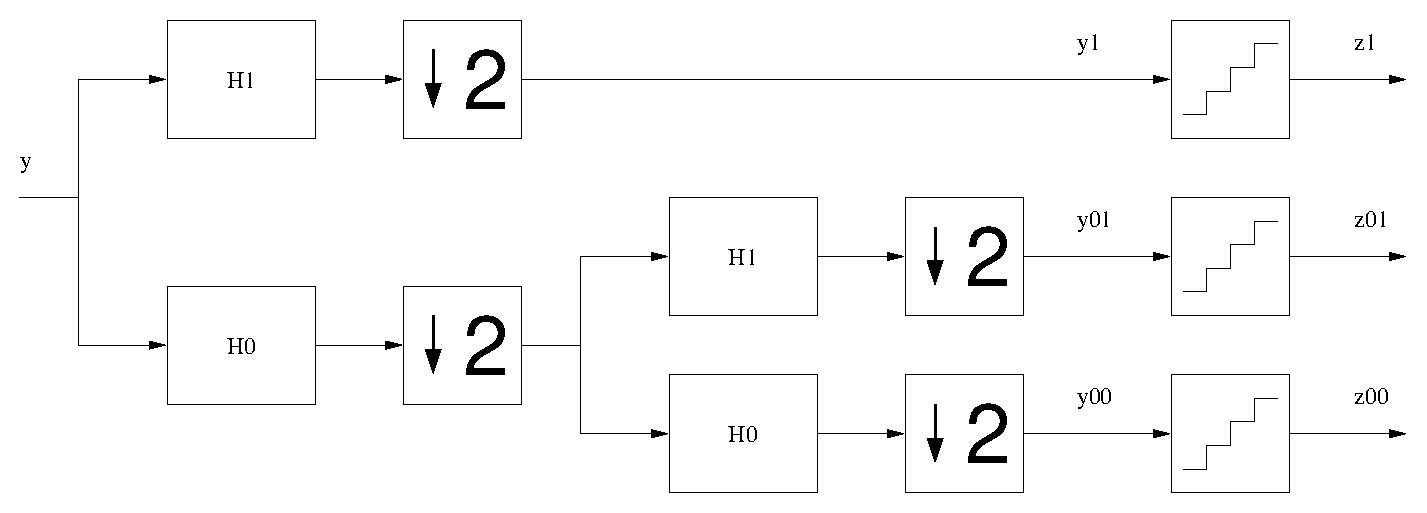
\includegraphics[height=4cm]{analysisbank3}
%    \caption{Analysis filter bank followed by quantization.}
%    \label{fig:analysisbank3}
%    \bigskip\bigskip
%    \psfrag{G0}[][]{$G_0(z)$}
%    \psfrag{G1}[][]{$G_1(z)$}
%    \psfrag{v}[][]{$v(n)$}
%    \psfrag{zl}[][]{$z^{-l}$}
%    \psfrag{z1}[r][r]{$z_1(n)$}
%    \psfrag{z01}[r][r]{$z_{01}(n)$}
%    \psfrag{z00}[r][r]{$z_{00}(n)$}
%    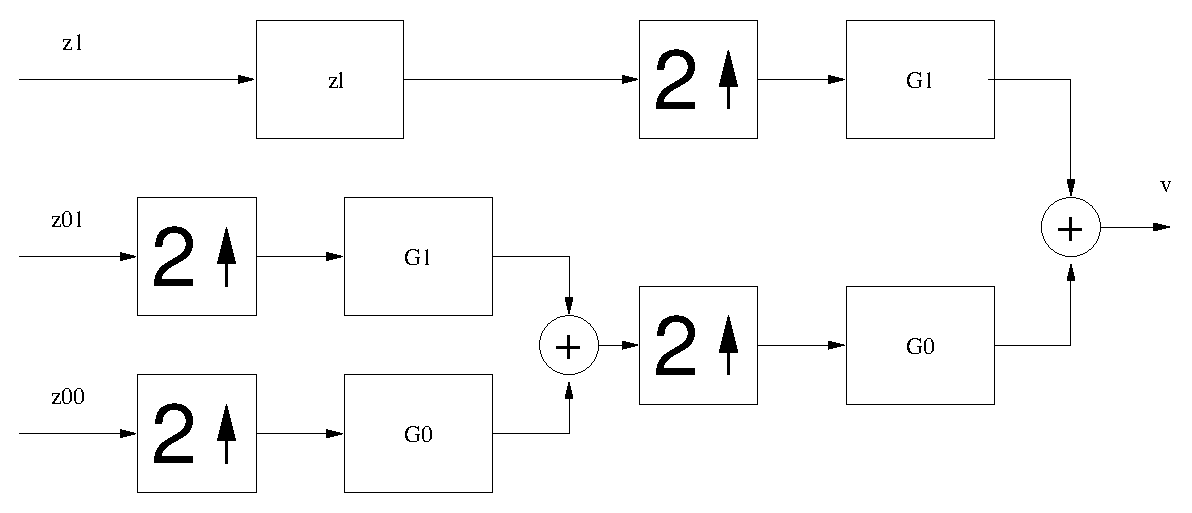
\includegraphics[height=4cm]{synthesisbank3}
%    \caption{Synthesis filter bank.}
%    \label{fig:synthesisbank3}
%  \end{center}
%\end{figure*}

\begin{thebibliography}{99}
\bibitem{latexmanual} Tobias Oetiker et al. \textsl{The Not So Short
    Introduction to
    \LaTeXe}
    www.tex.ac.uk/tex-archive/info/lshort/english/lshort.pdf
\end{thebibliography}
\end{document}
